\chapter{Perubahan yang Tidak Dapat Dibalik}\label{ch:g5:irreversible-changes}

Sebutir telur dipecahkan ke wajan panas. Dalam beberapa detik, putih
telur yang bening dan encer menjadi padat dan putih, dan kuningnya
mengental. Angkat wajan dari kompor, biarkan telurnya dingin, simpan di
lemari es: telur itu tidak akan pernah menjadi telur mentah lagi. Ada
perubahan yang dapat dibalik dan ada yang tidak. Membedakan keduanya
adalah langkah pertama ilmu kimia.

\begin{recall}
Padatan yang \omterm{def:g2:mixing-and-dissolving:dissolve}{larut} dalam air masih ada: ketika airnya mengering, padatan
itu tertinggal (\cref{ch:g2:mixing-and-dissolving}). \omterm{def:g4:what-a-fire-needs:burning}{Pembakaran}
menghasilkan zat-zat baru --- abu, asap, karbon dioksida, uap air ---
dan \omterm{def:g4:what-a-fire-needs:fuel}{bahan bakarnya} hilang untuk selamanya (\cref{ch:g4:what-a-fire-needs}).
\end{recall}

\begin{omfigure}
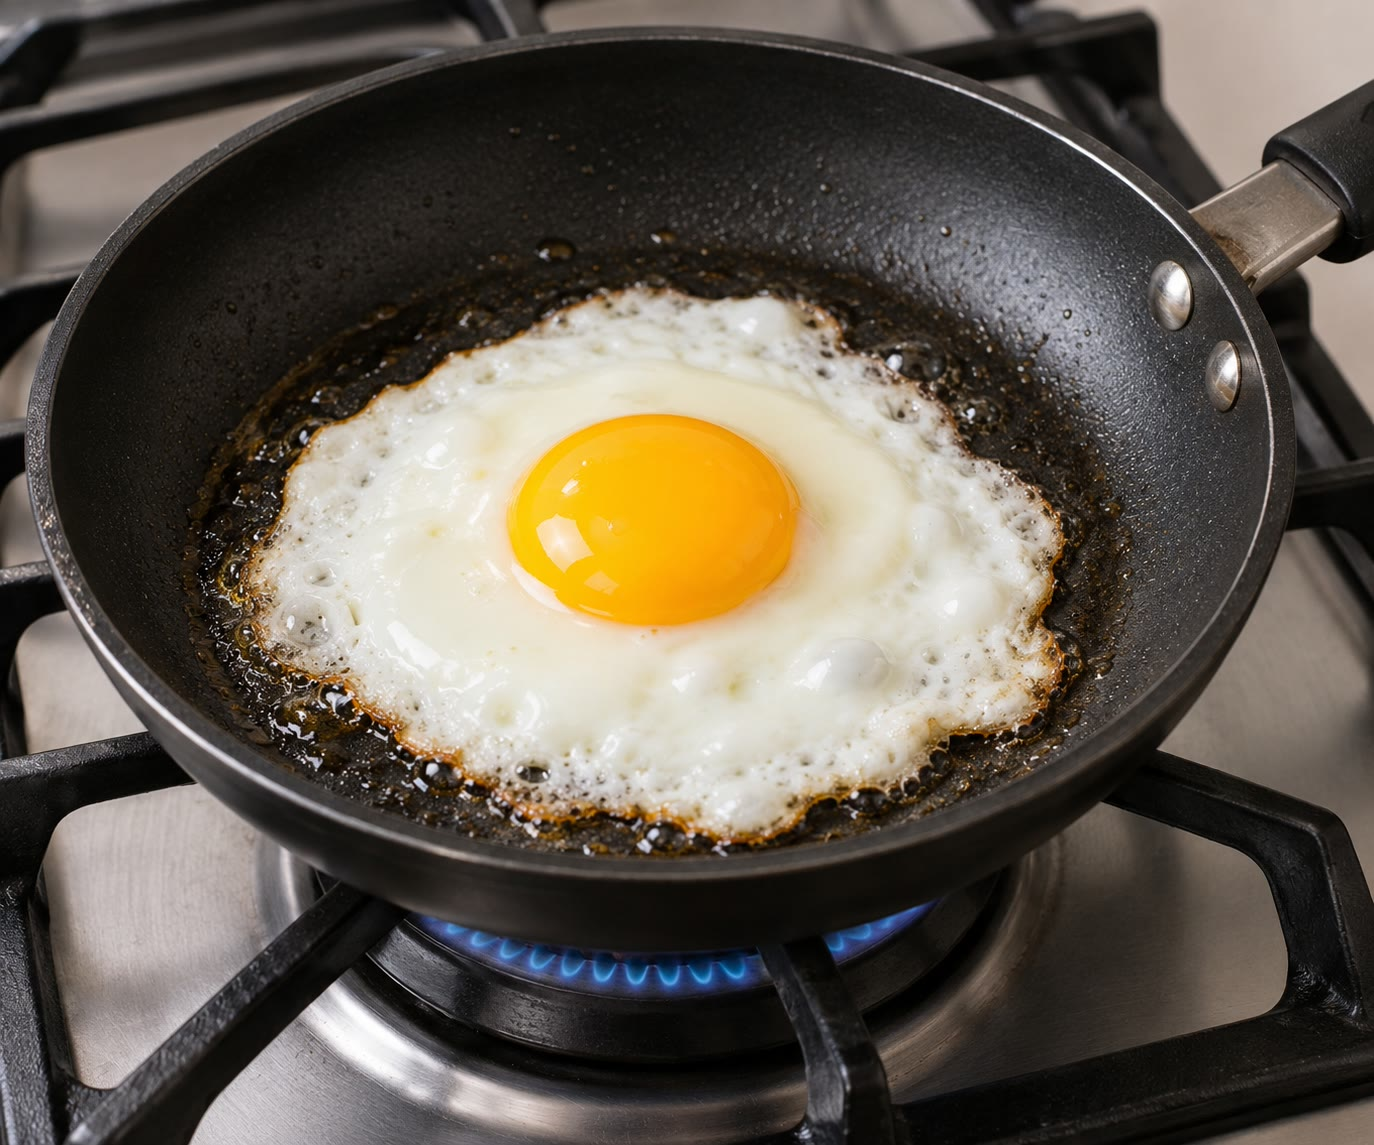
\includegraphics[width=0.55\linewidth]{images/book1/ai/g5-egg-frying.jpg}

{\small Telur yang sedang digoreng: putih telur yang bening telah menjadi
padat dan putih, untuk selamanya.}
\end{omfigure}

\section{Perubahan yang dapat dibalik}

\begin{definition}[Perubahan dapat balik]\label{def:g5:irreversible-changes:reversible}
Sebuah \emph{perubahan dapat balik}\index{perubahan dapat balik} adalah
perubahan yang dapat dibalik, sehingga kita memperoleh kembali tepat apa
yang ada di awal.
\end{definition}

\begin{example}[Melarutkan dan mengeringkan]\label{ex:g5:irreversible-changes:dissolve}
Gula yang diaduk ke dalam air akan \omterm{def:g2:mixing-and-dissolving:dissolve}{larut}. Biarkan airnya \omterm{def:g3:separating-mixtures:evaporate}{menguap}, dan
gulanya kembali: gula yang sama, semanis sebelumnya. Melarutkan adalah
\omterm{def:g5:irreversible-changes:reversible}{perubahan dapat balik}.
\end{example}

\begin{example}[Es dan air]\label{ex:g5:irreversible-changes:ice}
Es batu mencair menjadi air di atas piring yang hangat; masukkan air itu
ke dalam pembeku dan air itu menjadi es lagi. Mencair dan membeku adalah
\omterm{def:g5:irreversible-changes:reversible}{perubahan dapat balik}. (Mengapa air mencair dan membeku diceritakan di
buku fisika.)
\end{example}

\begin{example}[Mencampur]\label{ex:g5:irreversible-changes:mix}
Pasir yang \omterm{def:g2:mixing-and-dissolving:mix}{dicampur} kerikil dapat dipisahkan lagi dengan ayakan; air
berlumpur dapat disaring. \omterm{def:g2:mixing-and-dissolving:mix}{Mencampur} adalah \omterm{def:g5:irreversible-changes:reversible}{perubahan dapat balik}: tidak
ada yang baru terbentuk, dan bagian-bagiannya dapat dipisahkan
(\cref{ch:g3:separating-mixtures}).
\end{example}

\section{Perubahan yang tidak dapat dibalik}

\begin{definition}[Perubahan tak dapat balik dan perubahan kimia]\label{def:g5:irreversible-changes:chemical-change}
Sebuah \emph{perubahan tak dapat balik}\index{perubahan tak dapat balik}
adalah perubahan yang tidak dapat dibalik begitu saja. Kebanyakan di
antaranya adalah perubahan yang memunculkan zat-zat baru yang tidak ada
di awal: perubahan seperti itu disebut
\emph{perubahan kimia}\index{perubahan kimia}.
\end{definition}

\begin{example}[Enam perubahan kimia]\label{ex:g5:irreversible-changes:six}
\begin{itemize}
  \item \textbf{Memasak telur}: putih telur yang encer dan bening
        menjadi padat dan putih.
  \item \textbf{Memanggang kue}: adonan yang encer menjadi kue yang
        empuk berongga, cokelat di bagian luar, dengan bau yang baru.
  \item \textbf{\omterm{def:g4:what-a-fire-needs:burning}{Pembakaran}}: kayu menjadi abu, asap, karbon dioksida,
        dan uap air.
  \item \textbf{Perkaratan}: besi mengilap yang dibiarkan kehujanan
        menjadi tertutup zat jingga kecokelatan yang mudah mengelupas,
        yaitu karat.
  \item \textbf{Susu yang menjadi asam}: kalau terlupakan berhari-hari,
        susu mengental, menggumpal, dan berbau asam.
  \item \textbf{Apel yang dipotong menjadi cokelat}: daging buahnya yang
        pucat berubah cokelat di \omterm{def:g4:air-a-mixture-of-gases:air}{udara} dalam waktu satu jam.
\end{itemize}
Dalam setiap kasus, sesuatu yang baru telah terbentuk, dan tidak ada
cara sederhana untuk mendapatkan kembali apa yang ada di awal.
\end{example}

\begin{omfigure}
\begin{minipage}[t]{0.48\linewidth}\centering
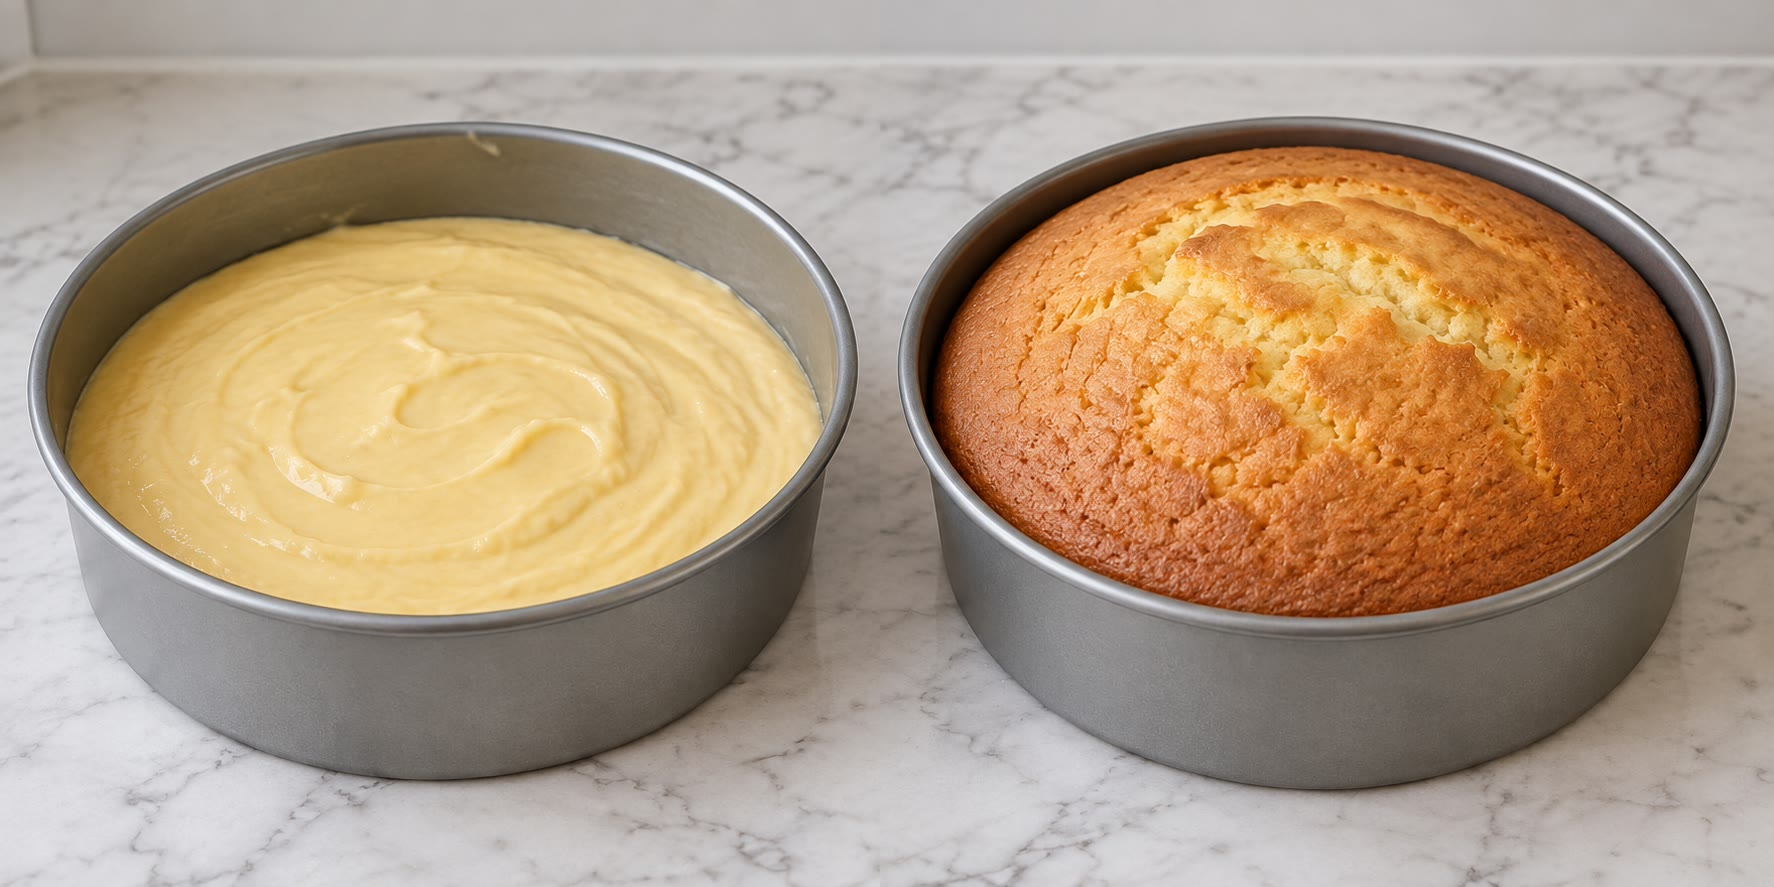
\includegraphics[width=\linewidth,height=4.6cm,keepaspectratio]{images/book1/ai/g5-cake-before-after.jpg}

{\small Adonan sebelum, kue sesudah: memanggang tidak dapat dibalik.}
\end{minipage}\hfill
\begin{minipage}[t]{0.48\linewidth}\centering
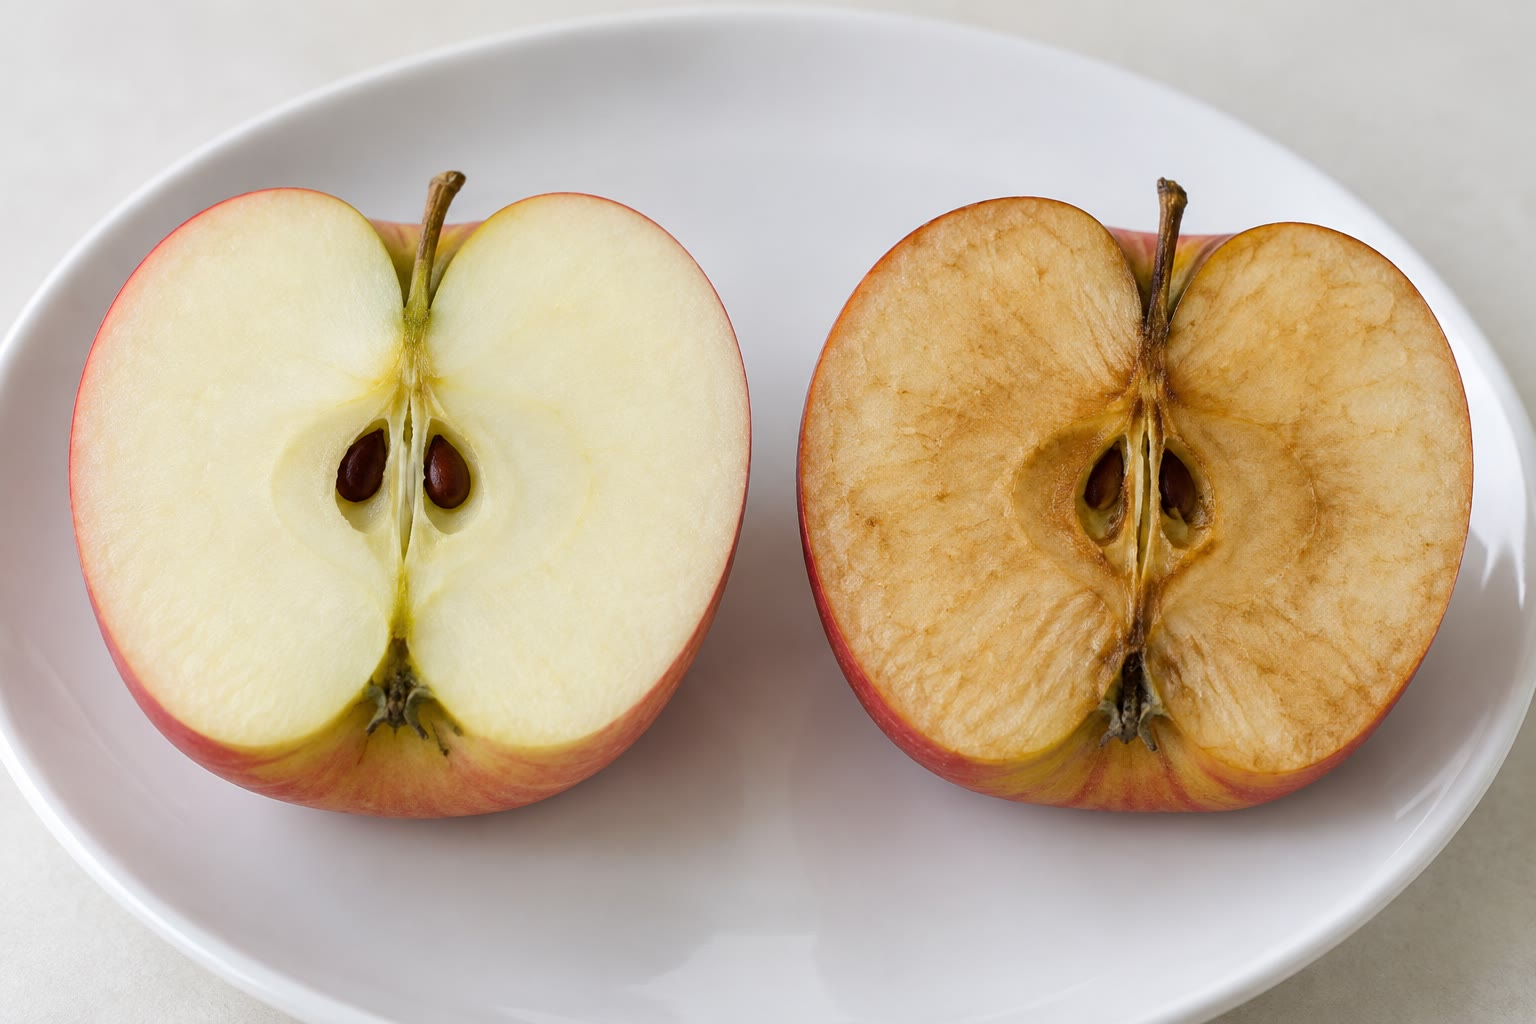
\includegraphics[width=\linewidth,height=4.6cm,keepaspectratio]{images/book1/ai/g5-apple-browning.jpg}

{\small Separuh apel yang segar dan separuh yang dibiarkan sejam di \omterm{def:g4:air-a-mixture-of-gases:air}{udara}.}
\end{minipage}
\end{omfigure}

\begin{omfigure}
\begin{tikzpicture}[font=\small]
  \node[font=\small\bfseries, omDef] at (2.7,4.6) {dapat dibalik};
  \node[font=\small\bfseries, omProp] at (9.6,4.6) {tidak dapat dibalik};
  \draw[black!30] (6.1,4.9) -- (6.1,-0.3);
  % reversible pairs
  \foreach \y/\a/\b in {3.6/{gula + air}/{air gula}, 2.0/{es}/{air cair},
                        0.4/{pasir + kerikil}/{campuran}} {
    \node[draw=omDef, fill=omDef!6, rounded corners=2pt, minimum width=2.3cm,
      minimum height=0.8cm] at (0.9,\y) {\a};
    \node[draw=omDef, fill=omDef!6, rounded corners=2pt, minimum width=2.3cm,
      minimum height=0.8cm] at (4.6,\y) {\b};
    \draw[->, thick, omDef] (2.3,\y+0.12) -- (3.25,\y+0.12);
    \draw[<-, thick, omDef] (2.3,\y-0.12) -- (3.25,\y-0.12);
  }
  % irreversible ones
  \foreach \y/\a/\b in {3.6/{telur mentah}/{telur matang}, 2.0/{kayu}/{abu, asap, gas},
                        0.4/{besi}/{karat}} {
    \node[draw=omProp, fill=omProp!6, rounded corners=2pt, minimum width=2.0cm,
      minimum height=0.8cm] at (7.6,\y) {\a};
    \node[draw=omProp, fill=omProp!6, rounded corners=2pt, minimum width=2.9cm,
      minimum height=0.8cm] at (11.5,\y) {\b};
    \draw[->, thick, omProp] (8.8,\y) -- (9.85,\y);
  }
\end{tikzpicture}

{\small Kiri: \omterm{def:g5:irreversible-changes:reversible}{perubahan dapat balik}; panah ganda menyatakan bahwa
perubahan itu dapat berlangsung ke dua arah. Kanan: \omterm{def:g5:irreversible-changes:chemical-change}{perubahan kimia},
hanya satu arah.}
\end{omfigure}

\section{Petunjuk bahwa zat baru telah muncul}

\begin{method}[Perubahan kimiakah? Carilah petunjuknya]\label{met:g5:irreversible-changes:clues}
Zat baru sering ditandai oleh salah satu petunjuk berikut:
\begin{enumerate}
  \item \textbf{warna} baru (warna cokelat pada roti panggang);
  \item \textbf{gelembung} gas yang muncul di dalam cairan tanpa
        dipanaskan (cuka yang dituang ke soda kue);
  \item \textbf{bau} baru (susu basi, roti gosong);
  \item \textbf{panas atau cahaya} yang dilepaskan (lilin yang
        menyala);
  \item \textbf{padatan yang muncul} di dalam cairan bening, atau
        gumpalan yang terbentuk (susu yang menggumpal).
\end{enumerate}
Satu petunjuk saja dapat menyesatkan: air yang mendidih bergelembung,
tetapi tidak ada yang baru terbentuk --- gelembung itu uap air, dan
airnya kembali ketika uap itu mendingin. Carilah beberapa petunjuk, dan
tanyakan: dapatkah perubahan itu dibalik?
\end{method}

\begin{omfigure}
\begin{tikzpicture}[font=\small]
  \foreach \k/\t in {0/{warna baru}, 1/{gelembung gas}, 2/{bau baru},
                     3/{panas atau cahaya}, 4/{muncul padatan}} {
    \begin{scope}[xshift=\k*3.2cm]
      \draw[omProp, line width=0.8pt, fill=omProp!5] (0,0) circle (1.0);
      \node[anchor=north, align=center] at (0,-1.15) {\t};
    \end{scope}
  }
  % 1: colour, a slice of toast half brown
  \fill[yellow!20, draw=brown!60] (-0.55,-0.5) rectangle (0.55,0.55);
  \fill[brown!55] (0,-0.5) rectangle (0.55,0.55);
  % 2: bubbles in a beaker
  \begin{scope}[xshift=3.2cm]
    \pic[transform shape, scale=0.45] at (0,-0.55) {beaker={0.7}{omWater!80}};
    \foreach \x/\y in {-0.15/-0.2,0.1/0.05,-0.05/0.25,0.18/-0.35,-0.2/0.15}
      \draw[black!55] (\x,\y) circle (0.05);
  \end{scope}
  % 3: smell, wavy lines
  \begin{scope}[xshift=6.4cm]
    \foreach \x in {-0.35,0,0.35} \draw[black!55, line width=0.8pt, decorate,
      decoration={snake, amplitude=1.5pt, segment length=6pt}] (\x,-0.6) -- (\x,0.6);
  \end{scope}
  % 4: a flame
  \begin{scope}[xshift=9.6cm]
    \fill[orange!80] (0,-0.6) .. controls (-0.45,-0.05) and (-0.15,0.35) .. (0,0.7)
      .. controls (0.15,0.35) and (0.45,-0.05) .. (0,-0.6);
    \fill[yellow!80] (0,-0.45) .. controls (-0.2,-0.1) and (-0.08,0.15) .. (0,0.3)
      .. controls (0.08,0.15) and (0.2,-0.1) .. (0,-0.45);
  \end{scope}
  % 5: solid settling in a test tube
  \begin{scope}[xshift=12.8cm]
    \pic[transform shape, scale=0.4] at (0,-0.65) {testtube={0.75}{omWater!80}};
    \fill[white, draw=black!40] (-0.08,-0.62) rectangle (0.08,-0.5);
    \foreach \x/\y in {-0.04/-0.3,0.04/-0.1,0/0.1} \fill[black!35] (\x,\y) circle (0.03);
  \end{scope}
\end{tikzpicture}

{\small Lima petunjuk bahwa mungkin telah terjadi \omterm{def:g5:irreversible-changes:chemical-change}{perubahan kimia}.}
\end{omfigure}

\begin{inthelab}[Cuka pada soda kue]
Guru menaruh sesendok soda kue, serbuk putih, di dasar sebuah gelas
kimia lalu menuangkan sedikit cuka. Campuran itu langsung berdesis dan
berbuih: gas dilepaskan, sebuah petunjuk \omterm{def:g5:irreversible-changes:chemical-change}{perubahan kimia}. Ketika
desisnya berhenti, soda kuenya sudah habis dan tidak dapat diperoleh
kembali dengan pengeringan.
\end{inthelab}

\begin{omfigure}
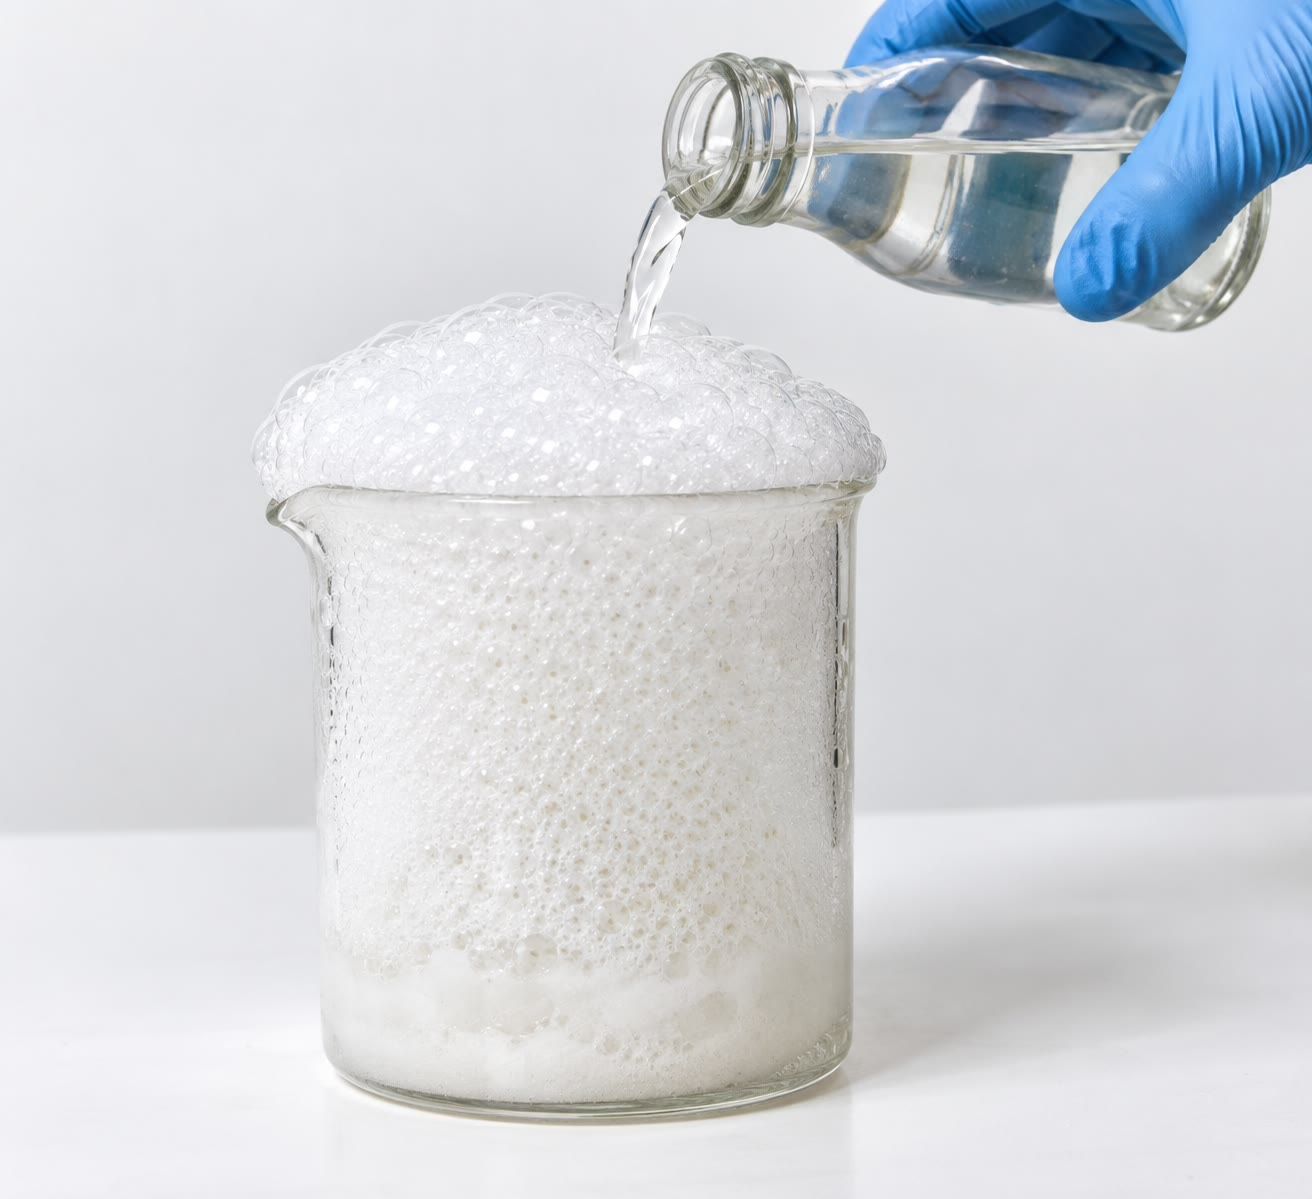
\includegraphics[width=0.5\linewidth]{images/book1/ai/g5-baking-soda-lab.jpg}

{\small Cuka pada soda kue: gas dilepaskan.}
\end{omfigure}

\section{Perubahan yang berguna dan yang merugikan}

\begin{proposition}[Perubahan kimia di sekitar kita]\label{prop:g5:irreversible-changes:around}
Banyak \omterm{def:g5:irreversible-changes:chemical-change}{perubahan kimia} yang berguna: memasak makanan, memanggang roti,
membakar gas untuk menghangatkan rumah, gips atau semen yang mengeras.
Ada pula yang merusak: besi yang berkarat, makanan yang basi, kayu yang
membusuk. Kita tidak dapat membaliknya, tetapi kita dapat
memperlambatnya:
\begin{itemize}
  \item makanan lebih awet di dalam dinginnya lemari es;
  \item cat atau lapisan minyak menjauhkan \omterm{def:g4:air-a-mixture-of-gases:air}{udara} dan air dari besi;
  \item apel yang dipotong lalu diperciki air jeruk lemon lebih lambat
        menjadi cokelat.
\end{itemize}
\end{proposition}

\begin{omfigure}
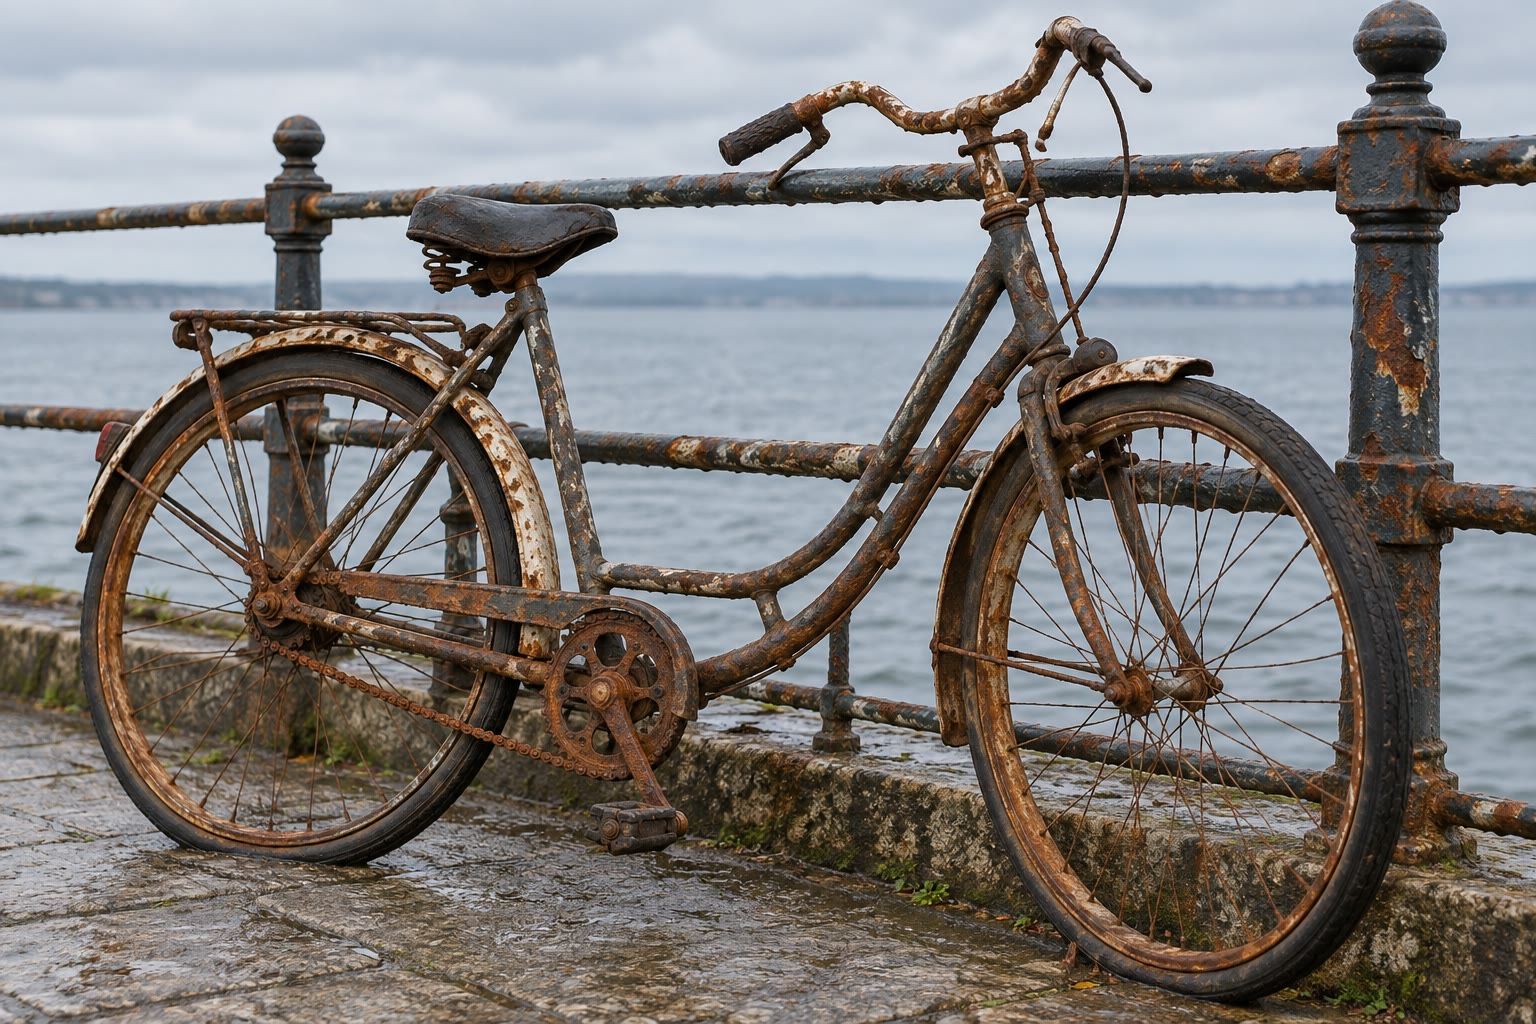
\includegraphics[width=0.55\linewidth]{images/book1/ai/g5-rusty-bicycle.jpg}

{\small Sepeda yang bertahun-tahun dibiarkan kehujanan: besinya telah
berkarat.}
\end{omfigure}

\begin{remark}[Dapat dibalik, tetapi tidak begitu saja]\label{rem:g5:irreversible-changes:not-simply}
``Tidak dapat dibalik'' berarti tidak ada jalan kembali yang sederhana,
seperti mendinginkan atau mengeringkan. Para ahli kimia kadang dapat
mengubah karat kembali menjadi besi, tetapi hanya dengan tanur dan
zat-zat baru: itu \omterm{def:g5:irreversible-changes:chemical-change}{perubahan kimia} yang lain, bukan pembalikan.
\end{remark}

\section{Latihan}

\begin{exercise}[$\star$]\label{exo:g5:irreversible-changes:1}
Katakan apakah setiap perubahan berikut dapat dibalik: cokelat yang
mencair, korek api yang \omterm{def:g4:what-a-fire-needs:burning}{terbakar}, garam yang dilarutkan dalam air, roti
yang dipanggang.
\end{exercise}

\begin{exercise}[$\star$]\label{exo:g5:irreversible-changes:2}
Apa itu \omterm{def:g5:irreversible-changes:chemical-change}{perubahan kimia}? Berikan dua contoh dari dapur.
\end{exercise}

\begin{exercise}[$\star$]\label{exo:g5:irreversible-changes:3}
Garam dilarutkan dalam air. Bagaimana garam itu dapat diperoleh
kembali? Apakah melarutkan merupakan \omterm{def:g5:irreversible-changes:reversible}{perubahan dapat balik}?
\end{exercise}

\begin{exercise}[$\star$]\label{exo:g5:irreversible-changes:4}
Petunjuk \omterm{def:g5:irreversible-changes:chemical-change}{perubahan kimia} apa yang kamu perhatikan ketika susu menjadi
asam? Sebutkan dua.
\end{exercise}

\begin{exercise}[$\star$]\label{exo:g5:irreversible-changes:5}
Lihatlah gambar dengan dua kolom. Perubahan mana yang memiliki panah
ganda? Apa arti panah ganda itu?
\end{exercise}

\begin{exercise}[$\star$]\label{exo:g5:irreversible-changes:6}
Mengapa rantai sepeda diberi minyak? \omterm{def:g5:irreversible-changes:chemical-change}{Perubahan kimia} apa yang
diperlambat oleh minyak itu?
\end{exercise}

\begin{exercise}[$\star$]\label{exo:g5:irreversible-changes:7}
Ketika cuka dituang ke soda kue, campuran itu berdesis. Petunjuk apakah
ini?
\end{exercise}

\begin{exercise}[$\star$]\label{exo:g5:irreversible-changes:8}
Sebutkan satu \omterm{def:g5:irreversible-changes:chemical-change}{perubahan kimia} yang berguna dan satu yang merugikan.
\end{exercise}

\begin{exercise}[$\star$]\label{exo:g5:irreversible-changes:9}
Mengapa kita menyimpan susu di lemari es?
\end{exercise}

\begin{exercise}[$\star\star$]\label{exo:g5:irreversible-changes:10}
Air bergelembung ketika mendidih. Apakah mendidih itu \omterm{def:g5:irreversible-changes:chemical-change}{perubahan kimia}?
Jelaskan mengapa satu petunjuk saja tidak cukup.
\end{exercise}

\begin{exercise}[$\star\star$]\label{exo:g5:irreversible-changes:11}
Tom berkata: ``Ketika lilin menyala, lilinnya hanya mencair dan habis,
seperti es.'' Pakailah dua petunjuk untuk menjelaskan mengapa lilin yang
menyala adalah \omterm{def:g5:irreversible-changes:chemical-change}{perubahan kimia}, dan bukan sekadar mencair.
\end{exercise}
